% !TeX spellcheck = en_GB
%%%%%%%%%%%%%%%%%%%%%%%%%%%%%%%%%%%%%%%%%
% Masters/Doctoral Thesis 
% LaTeX Template
% Version 2.5 (27/8/17)
%
% This template was downloaded from:
% http://www.LaTeXTemplates.com
%
% Version 2.x major modifications by:
% Vel (vel@latextemplates.com)
%
% This template is based on a template by:
% Steve Gunn (http://users.ecs.soton.ac.uk/srg/softwaretools/document/templates/)
% Sunil Patel (http://www.sunilpatel.co.uk/thesis-template/)
%
% Template license:
% CC BY-NC-SA 3.0 (http://creativecommons.org/licenses/by-nc-sa/3.0/)
%
%%%%%%%%%%%%%%%%%%%%%%%%%%%%%%%%%%%%%%%%%

%----------------------------------------------------------------------------------------
%	PACKAGES AND OTHER DOCUMENT CONFIGURATIONS
%----------------------------------------------------------------------------------------

\documentclass[
11pt, % The default document font size, options: 10pt, 11pt, 12pt
oneside, %TODO: % Two side (alternating margins) for binding by default, uncomment to switch to one side
english, % ngerman for German
singlespacing, % Single line spacing, alternatives: onehalfspacing or doublespacing
%draft, % Uncomment to enable draft mode (no pictures, no links, overfull hboxes indicated)
%nolistspacing, % If the document is onehalfspacing or doublespacing, uncomment this to set spacing in lists to single
liststotoc, % Uncomment to add the list of figures/tables/etc to the table of contents
toctotoc, % Uncomment to add the main table of contents to the table of contents
%parskip, % Uncomment to add space between paragraphs
%nohyperref, % Uncomment to not load the hyperref package
headsepline, % Uncomment to get a line under the header
%chapterinoneline, % Uncomment to place the chapter title next to the number on one line
consistentlayout, % Uncomment to change the layout of the declaration, abstract and acknowledgements pages to match the default layout
]{./latex_template} % The class file specifying the document structure

%\usepackage[utf8]{inputenc} % Required for inputting international characters
\usepackage[T1]{fontenc} % Output font encoding for international characters
\usepackage{mathpazo} % Use the Palatino font by default
\usepackage{tabu}
\usepackage{diagbox}
\usepackage{rotating}
\usepackage{makecell}
\usepackage{float}
\usepackage{url}
\usepackage{pdfpages}
\usepackage[normalem]{ulem}
\usepackage[autostyle=true]{csquotes} % Required to generate language-dependent quotes in the bibliography

\newcommand*{\fullref}[1]{\hyperref[{#1}]{\ref*{#1} \nameref*{#1}}} % One single link

%----------------------------------------------------------------------------------------
%	MARGIN SETTINGS
%----------------------------------------------------------------------------------------

\geometry{
	paper=a4paper, % Change to letterpaper for US letter
	inner=2.5cm, % Inner margin
	outer=3.8cm, % Outer margin
	bindingoffset=.5cm, % Binding offset
	top=1.5cm, % Top margin
	bottom=1.5cm, % Bottom margin
	%showframe, % Uncomment to show how the type block is set on the page
}
\global\tabulinesep=1.2mm

%----------------------------------------------------------------------------------------
%	Glossary SETTINGS
%----------------------------------------------------------------------------------------
\usepackage{hyperref}
\usepackage[toc,nopostdot, nonumberlist]{glossaries}%acronym
\setglossarystyle{altlist}
\usepackage{xparse}
\DeclareDocumentCommand{\newdualentry}{ O{} O{} m m m m } {
	\newglossaryentry{gls-#3}{
		name={#4 : #5},
		text={#5\glsadd{#3}},
		description={#6},
		#1
	}
	\makeglossaries
	\newacronym[see={[Siehe:]{gls-#3}},#2]{#3}{#4}{#5\glsadd{gls-#3}}
}
\renewcommand{\glstextformat}[1]{\textit{#1}}
\makeglossaries

\DeclareTextFontCommand{\emph}{\bfseries\em}

%----------------------------------------------------------------------------------------
%	THESIS INFORMATION
%----------------------------------------------------------------------------------------

\thesistitle{XMPP-Grid Broker} %is used in the title and abstract, print it elsewhere with \ttitle
\supervisor{Prof.~Dr.~Andreas~\textsc{Steffen}} %is used in the title page, print it elsewhere with \supname
\examiner{} %print it elsewhere with \examname
\author{Fabian~\textsc{Hauser} and Raphael~\textsc{Zimmermann}} %is used in the title page and abstract, print it elsewhere with \authorname

\keywords{XMPP Grid Broker} % is not currently used anywhere in the template, print it elsewhere with \keywordnames
\university{\href{https://www.hsr.ch}{University of Applied Sciences Rapperswil}} %is used in the title page and abstract, print it elsewhere with \univname
\department{Department of Computer Science} %is used in the title page and abstract, print it elsewhere with \deptname

\AtBeginDocument{
\hypersetup{pdftitle=\ttitle} % Set the PDF's title to your title
\hypersetup{pdfauthor=\authorname} % Set the PDF's author to your name
\hypersetup{pdfkeywords=\keywordnames} % Set the PDF's keywords to your keywords
}

\loadglsentries{glossar}

\begin{document}

\frontmatter % Use roman page numbering style (i, ii, iii, iv...) for the pre-content pages
\pagestyle{plain} % Default to the plain heading style until the thesis style is called for the body content

%----------------------------------------------------------------------------------------
%	TITLE PAGE
%----------------------------------------------------------------------------------------

\begin{titlepage}
\begin{center}

\vspace*{.06\textheight}
{\scshape\LARGE \univname\par} % University name

{\scshape\large Department of Computer Science\par}\vspace{1.2cm} % University name
\textsc{\Large Bachelor Thesis}\\[0.5cm] % Thesis type

\HRule \\[0.4cm] % Horizontal line
{\huge \bfseries \ttitle\par}\vspace{0.4cm} % Thesis title
\HRule \\[1.5cm] % Horizontal line
 
\begin{minipage}[t]{0.4\textwidth}
\begin{flushleft} \large
\emph{Authors:}\\
\authorname % Author name - remove the \href bracket to remove the link
\end{flushleft}
\end{minipage}
\begin{minipage}[t]{0.4\textwidth}
\begin{flushright} \large
\emph{Advisor:} \\
\supname \\[1cm]
\emph{External Co-Examiner:} \\
\examname \\[1cm]
\emph{Internal Co-Examiner:} \\
\textit{not yet defined} \\[1cm]
\end{flushright}
\end{minipage}\\[3cm]
 
\vfill

{\large Spring Term 2018}\\[4cm] % Date

\includegraphics{resources/logo_hsr} % University/department logo - uncomment to place it
 
\vfill
\end{center}
\end{titlepage}
%----------------------------------------------------------------------------------------
%	License / information PAGE
%------------------------------------------

\vspace*{\fill}

\noindent \textcopyright  Copyright 2018 by Fabian Hauser and Raphael Zimmermann\\

\noindent This documentation is available under the GNU FDL License. \\

\noindent The XMPP-Grid Broker software is licensed under the AGPL-License. This does not apply to third-party libraries.

\pagebreak

%----------------------------------------------------------------------------------------
%	QUOTATION PAGE
%----------------------------------------------------------------------------------------

\vspace*{0.1\textheight}

{\noindent\huge\textit{DON`T PANIC}\par\vspace{10pt}}

\noindent\enquote{\itshape It looked insanely complicated, and this was one of the reasons why the snug plastic cover it fitted into had the words DON`T PANIC printed on it in large friendly letters.}\bigbreak

\hfill The Hitchhiker`s Guide to the Galaxy

%----------------------------------------------------------------------------------------
%	ABSTRACT PAGE
%----------------------------------------------------------------------------------------

\begin{abstract}
\addchaptertocentry{\abstractname} % Add the abstract to the table of contents
\end{abstract}

%----------------------------------------------------------------------------------------
%	MANAGEMENT SUMMARY
%----------------------------------------------------------------------------------------

\chapter{Management Summary}
\addchaptertocentry{\abstractname} % Add the abstract to the table of contents
%The Thesis Management Summary is written here (and usually kept to just this page).
% Das Management Summary richtet sich in der Praxis an die "Chefs des Chefs",
%  d.h. an die Vorgesetzten des Auftraggebers (diese sind in der Regel keine Fachspezialisten).
%  Die Sprache soll knapp, klar und stark untergliedert sein. Zu verwenden ist folgenden Gliederung:
% - Ausgangslage
% - Vorgehen, Technologien
% - Ergebnisse
% - Ausblick (optional)

% prototype demonstrates feasability
% further conceptual refinement needed
% implemenetation is complex - but doable.

%----------------------------------------------------------------------------------------
%	ACKNOWLEDGEMENTS
%----------------------------------------------------------------------------------------

\begin{acknowledgements}
\addchaptertocentry{\acknowledgementname} % Add the acknowledgements to the table of contents
We would like to thank our advisor, Prof.~Dr.~Andreas~Steffen, for his continuous support and helpful comments.

\end{acknowledgements}

%----------------------------------------------------------------------------------------
%	LIST OF CONTENTS PAGES
%----------------------------------------------------------------------------------------

\setcounter{tocdepth}{2}
\tableofcontents % Prints the main table of contents

%----------------------------------------------------------------------------------------
%	DEDICATION
%----------------------------------------------------------------------------------------

%TODO
%\dedicatory{For/Dedicated to/To my\ldots}

%----------------------------------------------------------------------------------------
%	THESIS CONTENT - CHAPTERS
%----------------------------------------------------------------------------------------

\mainmatter % Begin numeric (1,2,3...) page numbering

\pagestyle{thesis} % Return the page headers back to the "thesis" style

% !TeX spellcheck = en_GB
\newcommand{\code}{\texttt}
\chapter{Introduction}
\label{sec:introduction}

In this chapter, we introduce the terminology and background of our thesis task, to conclude in the motivation and legitimisation of our thesis.

\section{Terminology}
Taking into account that the intended audience for this thesis are developers and operators of security reporting systems, 
we mostly use the  Security Automation and Continuous Monitoring (SACM) terminology~\cite{ietf-sacm-terminology-14}
and thereby follow the same guidelines as the XMPP grid draft~\cite{ietf-mile-xmpp-grid-05}.

\section{Background}

The following sections introduce the underlying XMPP protocol and the relevant extensions (\glspl{xep}) of the XMPP grid draft as well as a summary of it and the corresponding XMPP terminology.

\subsection{XMPP (eXtensible Messaging and Presence Protocol)}
The Extensible Messaging and Presence Protocol (in short \gls{xmpp}) is an open protocol that enables the near-real-time exchange of small data between any network endpoints, hereafter called \glspl{platform}~\cite{rfc6120}.
While it was originally designed as an Instant Messaging (IM) protocol, it can be used for a wide range of data exchange applications~\cite{ieee-xplore-stream-xml-xmpp}.

XMPP is made of small building blocks defined in the core protocol~\cite{rfc6120} and numerous extensions called \glspl{xep}~\cite{xep-0001}.
The core is comprised of functionality for setup and encryption of communication channels, \gls{xml} streams, error handling and more. Additional functionality such as \gls{service-discovery}~\cite{xep-0030} and \gls{publish-subscribe}~\cite{xep-0060} are defined in separate extensions.

Although XMPP supports peer-to-peer communication, it is often used in a traditional client-server architecture.
A client (\gls{platform}) can send data to any addressable entity (any other \glspl{platform}) using \Gls{jabber} Identifiers, hereafter called \gls{jid}. If the \gls{jid} of the receiver has a different domainpart than the current server (\gls{controller}), the message is forwarded to the responsible XMPP server under its domain~\cite{rfc6120}.

The data exchanged over XMPP is \gls{xml} which makes the protocol structured and extensible, but leads to some protocol overhead.
XMPP communicates over unidirectional data streams with a server, which are basically long-lived \gls{tcp} connections.
The client opens a channel to the server over this connection, and the server opens one back (i.e. \code{<stream>} XML tags). In both streams, an XML document is opened after the connection is established.
During the conversation, an arbitrary amount of \glspl{stanza} (specified XML child elements) are written to the stream.
Before a connection may be terminated, the root element is closed (i.e. \code{</stream>}) and both streams form valid XML documents~\cite{rfc6120}\cite{professional-xmpp}.

The core \gls{stanza} types are \glspl{message}~(\code{<message/>}), \gls{presence}~(\code{<presence/>}) and\\
\gls{info-query}~(\code{<iq/>}).
\Glspl{message} can contain arbitrary data similar to email but are optimised for immediate delivery.
\Gls{presence} \glspl{stanza} deal with network availability and the propagation of user presence information.
An \gls{info-query} \gls{stanza} consists of a request and response (similar to the GET and POST HTTP methods), which is used for feature negotiation, configuration and general information exchange.
Because of these coarse semantics, XMPP provides a generalized communication layer~\cite{rfc6120}\cite{ieee-xplore-stream-xml-xmpp}.

Figure~\ref{fig:xmpp-overview} illustrates an example setup with two servers and three clients.

\begin{figure}[h]
	\centering
	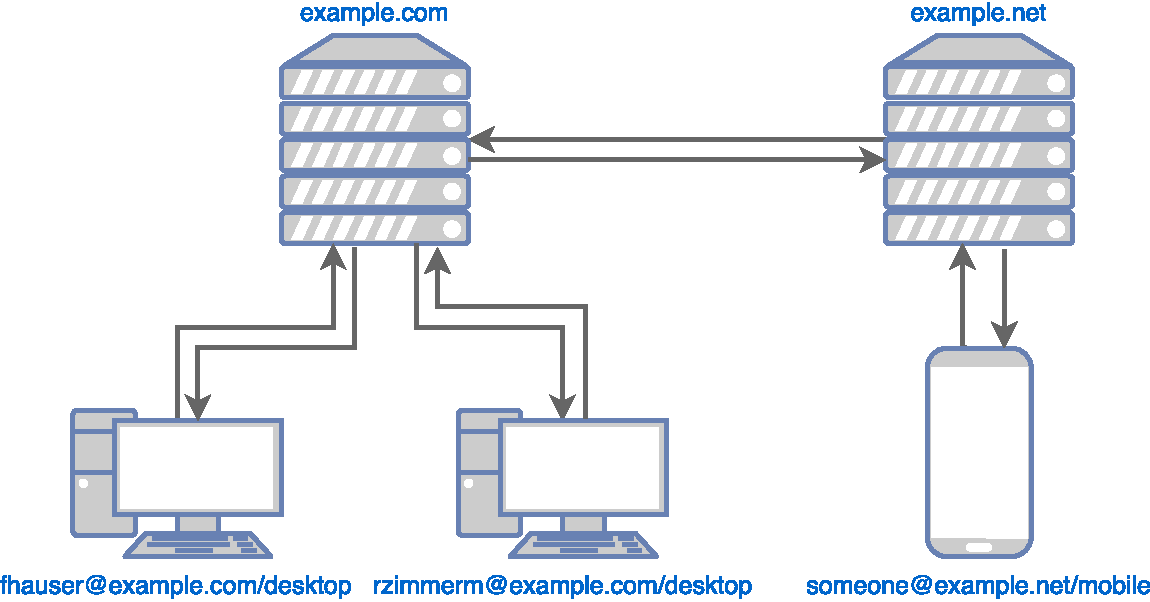
\includegraphics[width=0.8\linewidth]{resources/xmpp_overview.pdf}
	\caption{Two XMPP domains (servers), one with two users and one with one mobile user.}
	\label{fig:xmpp-overview}
\end{figure}

\subsection{Relevant XMPP Extensions}

The XMPP grid draft~\cite{ietf-mile-xmpp-grid-05} is based on multiple \glspl{xep}, most notably \gls{publish-subscribe}. In this section, we give an overview of the most relevant used \glspl{xep}.

\paragraph{XEP-0004: \gls{data-forms}} is a flexible protocol that can be used in workflows such as service configuration as well as for application-specific data description and reporting. The protocol provides form processing, common field types and extensibility mechanisms~\cite{xep-0004}.

\paragraph{XEP-0030: \gls{service-discovery}} enables entities to discover information about the identity and capabilities of other entities, e.g. whether the entity is a server or not, or items associated with an entity, e.g. a list of \gls{publish-subscribe} nodes~\cite{xep-0030}.

\paragraph{XEP-0059: \Gls{result-set-management}} allows entities to manage the receipt of large result sets, e.g. by paging through the result or limiting the number of results. \gls{result-set-management} is often desired when dealing with large dynamic result sets, as from service discovery or publish-subscribe, and time or other resources are limited~\cite{xep-0059}.

\subsubsection{XEP-0060: \Gls{publish-subscribe}}
The \gls{publish-subscribe} Extension, hereafter referred to as \gls{pubsub} or \gls{broker}, enables XMPP entities (\gls{provider}) to broadcast information via \glspl{topic} to subscribed entities (\gls{consumer})~\cite{xep-0060}.

Nodes, hereafter referred to as \glspl{topic}, are the communication hubs. Entities can create topics and configure them, e.g. set up subscription timeouts, limit publish and subscription rights. The configuration mechanism is based on data forms (XEP\babelhyphen{nobreak}0004).

The protocol defines a hierarchy of six affiliations of which only the implementation of `owner` and `none` is required. The implementation of the remaining four affiliations is recommended. An owner of a topic can manage the subscriptions and affiliations of other entities associated with a given topic.

To make the creation of topics simpler for clients, \gls{pubsub} defines five topic access models ("node access models"): open, presence, roaster, authorize and whitelist.

The open model allows uncontrolled access while presence and roaster are specific for IM. Using the authorize model, the owner has to approve all subscription requests. The whitelist model enables the owner to maintain a list of entities that are allowed to subscribe.

\subsection{IETF Internet-Draft: Using XMPP for Security Information Exchange}\label{sec:ietf-internet-draft-using-xmpp-for-security-information-exchange}
This IETF Internet draft describes how the XMPP protocol enhanced with the previously discussed XEPs, most notably the \gls{pubsub} extension, can be used for the exchange and distribution of security-relevant information between network devices.

One of the primary motivation for using XMPP for this task is the fast propagation of such security-relevant data.
Using XMPP for such a task also comes with its downsides. Most notably, because the XMPP server (\gls{broker}/\gls{controller}) is the central configuration component in charge of managing access permission, its compromisation has serious consequences.

The draft describes a trust model, thread model as well as specific countermeasures, e.g. to use at least TLS 1.2. These countermeasures also define restrictions of the XMPP protocol and its extensions, e.g. by limiting the topic access models of \gls{pubsub} to whitelist and authorized only~\cite{ietf-mile-xmpp-grid-05}.

\section{Motivation}
In this section, we legitimate this thesis and explain the value and applicability of our proposed solution.

\subsection{Present situation}
The IETF standard draft \emph{Using \gls{xmpp} for Security Information Exchange} \cite{ietf-mile-xmpp-grid-05} as summarised in section \ref{sec:ietf-internet-draft-using-xmpp-for-security-information-exchange} defines a protocol to exchange security-relevant information between endpoints.
The draft was created by the Managed Incident Lightweight Exchange (MILE) Working Group to support computer and network security incident management.

To demonstrate the viability of the draft a rapid prototype was developed in November~2017~\cite{xmpp-grid-prototype}.

\subsection{Problem and Solution}
Currently, there exists no implementation of the \gls{xmpp} grid draft management functionality which is ready for production use regarding usability and security.

To solve this problem, a graphical interface with bindings to a suitable \gls{broker} must be proposed and implemented.
The interface should permit network administrators to manage and review \glspl{topic}, persisted items and \glspl{platform}. Additionally, access and publishing permissions of \glspl{topic} and \glspl{platform} must be manageable.

\subsubsection*{} %This is needed, so that not the next page is referenced.
\label{lastpage} %TODO: This label should be positioned below above the last paragraph

\cleardoublepage
%----------------------------------------------------------------------------------------
%	BIBLIOGRAPHY
%----------------------------------------------------------------------------------------
\backmatter
\pagenumbering{Roman}

\bibliographystyle{abbrv}
\bibliography{references}
\addcontentsline{toc}{chapter}{Bibliography}


%----------------------------------------------------------------------------------------
%	LIST OF FIGURES/TABLES PAGES
%----------------------------------------------------------------------------------------

\listoffigures % Prints the list of figures

\listoftables % Prints the list of tables

%----------------------------------------------------------------------------------------
%	GLOSSARY
%----------------------------------------------------------------------------------------

\glsaddall
\printglossary


%----------------------------------------------------------------------------------------
%	THESIS CONTENT - APPENDICES
%----------------------------------------------------------------------------------------


\appendix % Cue to tell LaTeX that the following "chapters" are Appendices
\chapter{Appendices}
\setcounter{secnumdepth}{3}
\renewcommand{\thechapter}{A}
\section{Task Description}\label{sec:task-description}

\includepdf[pages=-,scale=.9,frame]{../task-description-signed.pdf}
\section{Project Plan}\label{sec:project-plan}
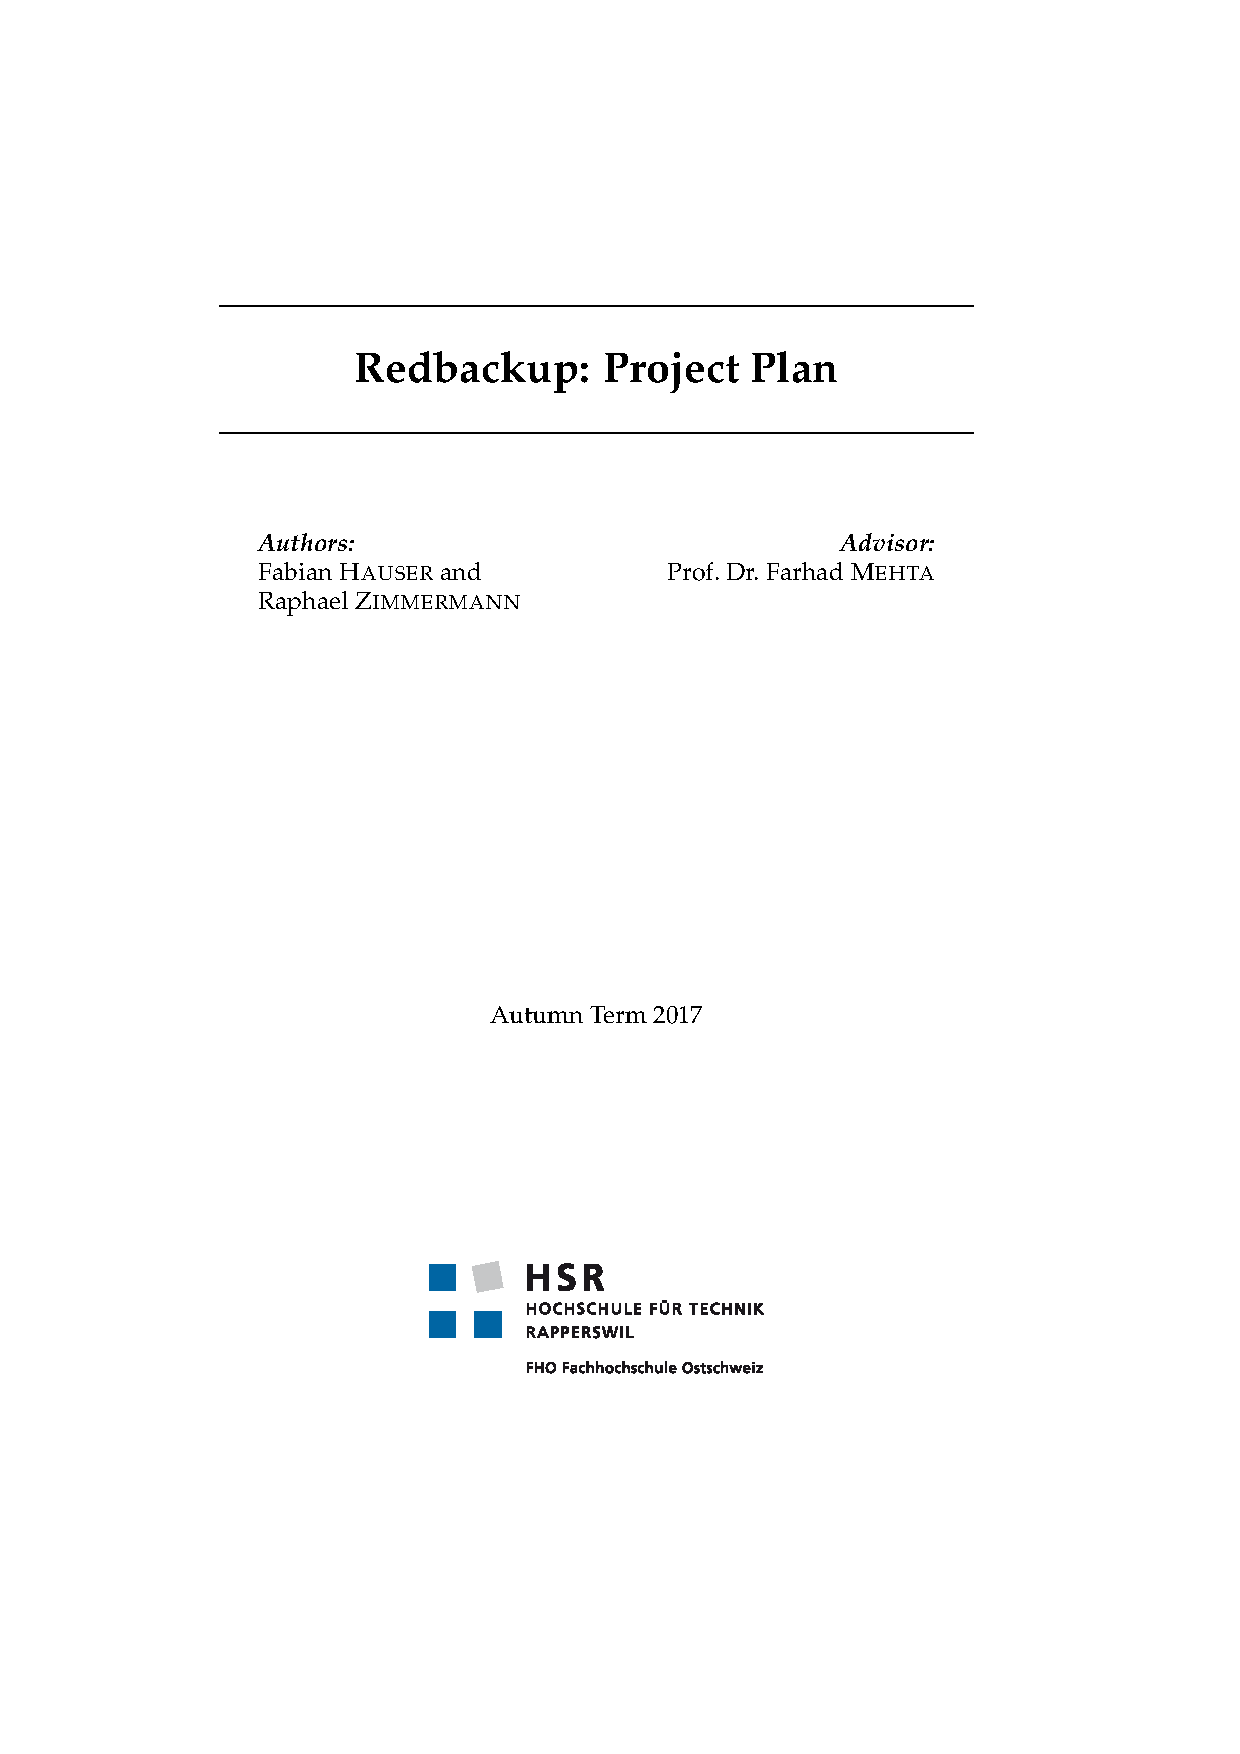
\includepdf[pages=-,scale=.9,frame]{../project-plan/project-plan.pdf}
\section{Development Guide}\label{sec:development-guide}
\includepdf[pages=-,scale=.9,frame]{../development-guide.pdf}
\section{Architectural Decisions}\label{sec:development-guide}
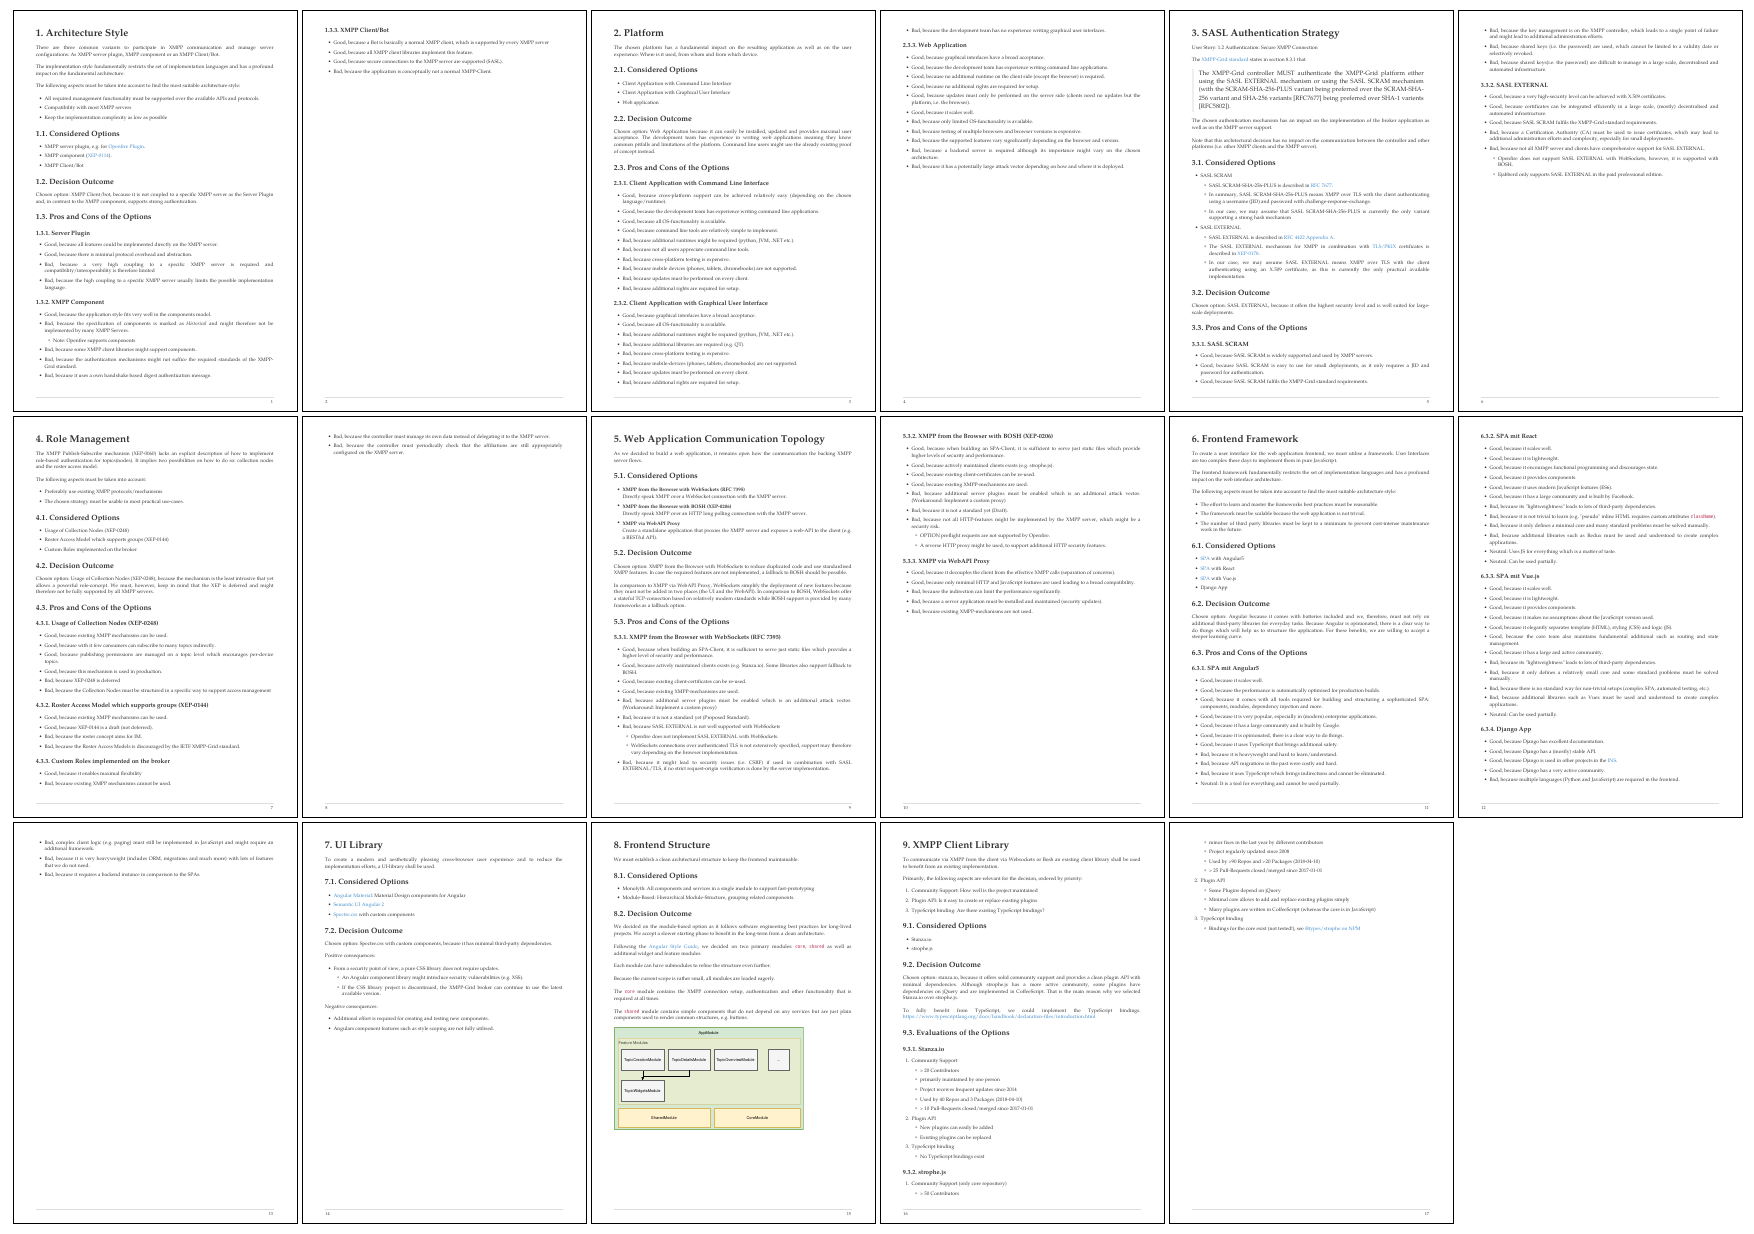
\includepdf[pages=-,scale=.9,frame]{../architectural-decisions/architectural-decisions.pdf}
\section{Time Accounting}\label{sec:time-accounting}

\includepdf[pages=-,scale=.9,frame]{../time-accounting.pdf}
\section{Meeting Minutes}\label{sec:meeting-minutes}
\includepdf[pages=-,scale=.9,frame]{../meeting-minutes/meeting-minutes.pdf}

% !TeX spellcheck = en_GB

\section{Requirements}\label{sec:requirements}

The following sections describe the primary requirements in the form of user stories~\cite{agile-alliance-user-stories}.
Figure~\ref{fig:requirements-overview} shows an overview of the primary use stories.

\begin{figure}[h]
    \centering
    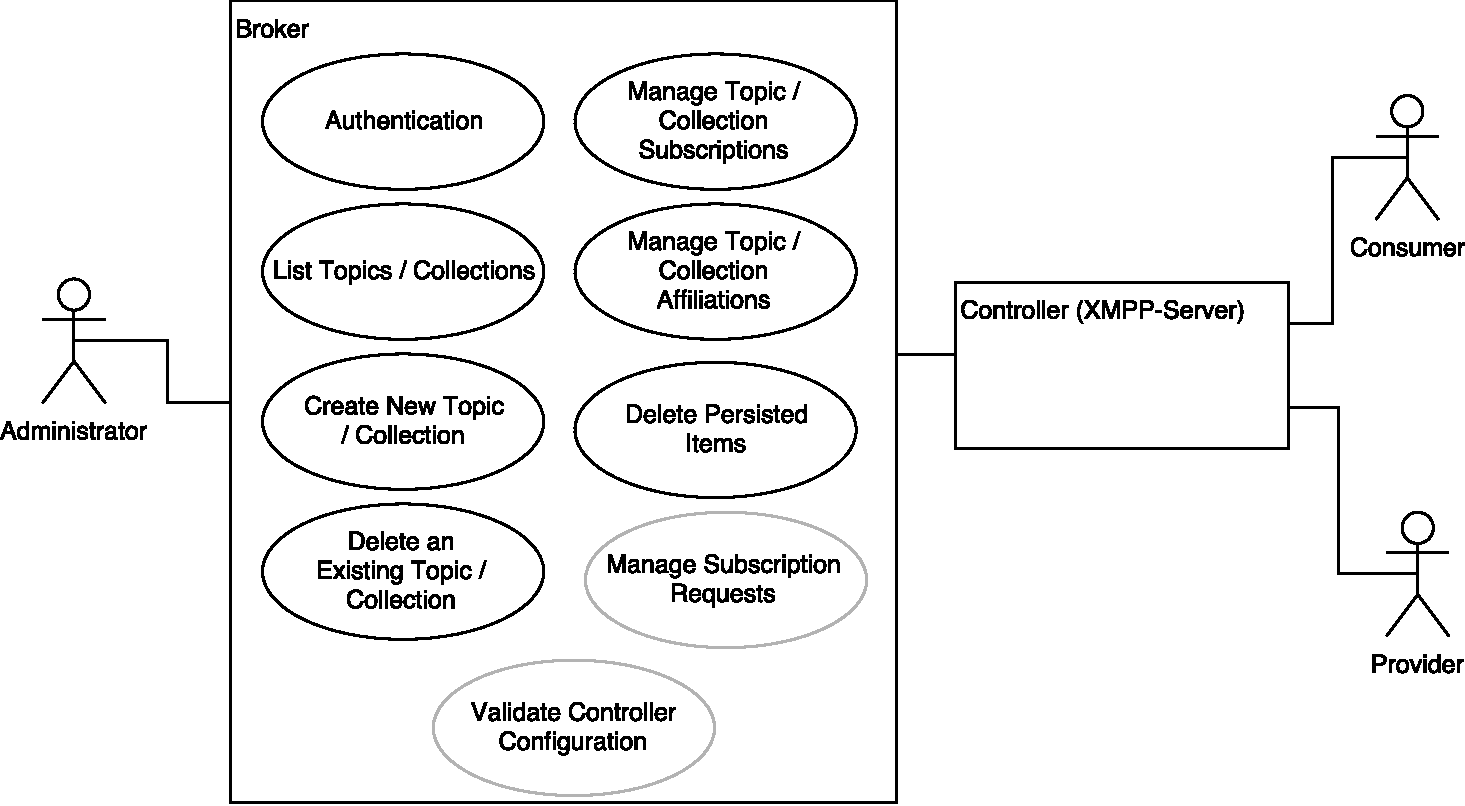
\includegraphics[width=1\linewidth]{resources/requirements_overview}
    \caption{UML use case diagram presenting an overview of the primary user stories.}
    \label{fig:requirements-overview}
\end{figure}

\subsection{Authentication}\label{sec:authentication}
\subsubsection{Login}

As an Administrator,\\
I want to log in\\
- preferably using an existing client \gls{tls} certificate - \\
so that only I can inspect and manage topics.\\

\subsubsection{Secure \gls{xmpp} Authentication}

As an Administrator concerned with security requirements,\\
I want to use either \gls{sasl-external} or \gls{sasl-scram} mechanism for authentication -

\begin{itemize}
    \item preferably the SCRAM-SHA-256-PLUS variant and
    \item preferably using mutual certificate-based authentication including revocation status checking
\end{itemize}

\noindent - so that the controller is fully compatible with the \gls{xmpp-grid} standard~\cite{ietf-mile-xmpp-grid-05}.

\noindent To achieve this goal, I am willing to accept:
\begin{itemize}
    \item More costly and less user friendly authentication
    \item limited compatibility of supported \gls{xmpp} servers
\end{itemize}

\subsubsection{Secure \gls{xmpp} Connection}

As an Administrator concerned with security requirements,\\
I want to use minimally \gls{tls} 1.2 [RFC5246] to communicate with the \gls{xmpp} server at all times\\
to achieve maximal security and compatibility with the \gls{xmpp-grid} standard~\cite{ietf-mile-xmpp-grid-05}.

\subsubsection{Secure Connection}

As an Administrator concerned with security requirements,\\
I want to use minimally \gls{tls} 1.2 [RFC5246] to communicate with the \gls{broker}\\
to achieve maximal security.

\subsubsection{Multiple Administrators}\label{sec:requirement-multiple-administrators}

As an Administrator,\\
I want to grant access to administrators \\
so that they can also manage the application.

\subsubsection{Audit Trail}\label{sec:requirement-audit-trail}

As an Administrator concerned with security requirements,\\
I want to be able to access an audit log\\
- preferably using existing \gls{xmpp} mechanisms - \\
so that I can reconstruct what other Administrations did on the controller.

\subsubsection{Logout}\label{sec:requirement-logout}

As an Administrator,\\
I want to log out\\
so that I can terminate a session.

\subsection{List Topics and Collections}\label{sec:list-topics}

\subsubsection{List All Topics}\label{sec:requirement-list-all-topics}
As an Administrator,\\
I want to see a list of all topics of the associated controller\\
so that I can quickly assimilate which topics exist.

\subsubsection{List All Top-Level-Collections}
As an Administrator,\\
I want to see a list of all top-level-collections of the associated controller\\
so that I can quickly assimilate which collections exist.

\subsubsection{List All Parent-Collections of a Topic}
As an Administrator,\\
I want to see a list of all transitive parent collections that contain a given topic\\
so that I can quickly assimilate in which collections items are published.

\subsubsection{List All Subtopics and Subcollection of a Collection}
As an Administrator,\\
I want to see a list of all collections and topics that a given collection contains\\
so that I can quickly assimilate the collection hierarchy.

\subsubsection{List Available topics With Limited Access (optional)}

As an Administrator,\\
I want to see a list of all topics of the associated controller to which I have limited access to,\\
to simplify troubleshooting and locate errors.

\subsubsection{List Available collections With Limited Access (optional)}

As an Administrator,\\
I want to see a list of all collections of the associated controller to which I have limited access to,\\
to simplify troubleshooting and locate errors.

\subsubsection{Topic and Collection Paging}
As an Administrator,\\
I want to be able to page through any set of collection/topic with more than 10 Items \\
so that I can work with more than 1000 collections and topics more effectively.

\subsubsection{Topic and Collection Name Filter}\label{sec:requirement-topic-filter}
As an Administrator,\\
I want to be able to quickly filter any set of collections/topics with more than 10 Items \\
so that I can work with more than 1000 collections and topics more effectively.

\subsection{Create a New Topic}\label{sec:create-topic}

As an Administrator,\\
I want to create a new topic on the associated controller\\
so that I am not tied to a fixed set of topics.

\subsection{Create a New Collection}\label{sec:create-collection}

As an Administrator,\\
I want to create a new collection on the associated controller\\
so that I can flexibly patch topics together.

\subsubsection{Override Default Topic Configuration}\label{sec:requirement-topic-default-configuration}

As an Administrator in the process of creating a new topic,\\
I want to override the default configuration (e.g. the affiliations) \\
so that I can restrict access and provide reasonable defaults.

\subsubsection{Override Default Collection Configuration}\label{sec:requirement-collection-default-configuration}

As an Administrator in the process of creating a new collection,\\
I want to override the default configuration (e.g. the affiliations) \\
so that I can restrict access and provide reasonable defaults.

\subsubsection{Initial topic Consumers and Providers}\label{sec:requirement-initial-topic-consumer-provider}

As an Administrator in the process of creating a new topic,\\
I want to specify an initial set of consumers and providers \\
so that I can restrict access to that topic and provide reasonable defaults.

\subsubsection{Initial Collection Consumers}\label{sec:requirement-initial-collection-consumer}

As an Administrator in the process of creating a new collection,\\
I want to specify an initial set of consumers \\
so that I can restrict access to that collection and provide reasonable defaults.

\subsection{Delete an Existing Topic}\label{sec:delete-topic}

As an Administrator,\\
I want to delete an existing topic on the associated controller\\
so that I can get rid of obsolete topics.

\subsection{Delete an Existing Collection}\label{sec:delete-collection}

As an Administrator,\\
I want to delete an existing collection on the associated controller\\
so that I can get rid of obsolete collections.


\subsubsection{Fault Prevention On Topic-Delete}

As an Administrator in the process of deleting a topic, \\
I want a mechanism to prevent me from deleting the wrong topic on the associated controller\\
(e.g. require me to enter the name of the topic manually).

\subsubsection{Fault Prevention On Collection-Delete}

As an Administrator in the process of deleting a collection, \\
I want a mechanism to prevent me from deleting the wrong collection on the associated controller\\
(e.g. require me to enter the name of the collection manually).


\subsection{Manage Topic/Collection Subscriptions}\label{sec:manage-subscriptions}

\subsubsection{List Consumers}

As an Administrator, \\
I want to list all consumers (including their JIDs) of a given topic/collection on the associated controller, \\
so that I can verify that specific consumers are subscribed, and others are not.


\subsubsection{Inspect Detailed Subscription Configuration}

As an Administrator, \\
I want to inspect the detailed topic/collection subscription configuration of a given consumer, \\
so that I can reproduce and reason about the receipt of data on that consumer
and find potential misconfiguration.

\subsubsection{Partially Modify Subscription Configuration}

As an Administrator, \\
I want to modify parts of the topic/collection subscription configuration of a given consumer, \\
so that I can fix misconfiguration.

\subsubsection{Unsubscribe Consumer}

As an Administrator, \\
I want to manually unsubscribe a specific consumer from a particular topic/collection on the associated controller, \\
so that I can remove obsolete or undesired subscriptions.

\subsubsection{Subscribe Consumer}

As an Administrator, \\
I want to manually subscribe a specific consumer on a particular topic/collection on the associated controller, \\
so that I can faster setup and manage consumers.

\subsection{Manage Topic Affiliations}\label{sec:manage-affiliations}
\subsubsection{Inspect Affiliations}

As an Administrator,\\
I want to list all Affiliations (JID and "Role") for a particular topic/collection on the associated controller \\
so that I can find potential misconfiguration.

\subsubsection{Modify Affiliations}

As an Administrator,\\
I want to modify the Affiliation ("Role") of a given JID for a particular topic/collection on the associated controller \\
so that I can fix potential misconfiguration.

\subsubsection{Fault Prevention When Modifying My Affiliation}

As an Administrator in the process of modifying my Affiliation for a particular topic/collection on the associated controller,\\
I want a mechanism to prevent me from accidentally downgrading my rights.

\subsubsection{Meaningful Error For Topics/Collection With Limited Access}

As an Administrator,\\
I want to receive a meaningful error message when inspecting a topic/collection to which I have limited access \\
so that I can quickly comprehend why the configuration options are limited.

\subsection{Manage Persisted Items of a Topic}\label{sec:manage-persisted-items}
\subsubsection{Inspect Persisted Items}

As an Administrator,\\
I want to list all persisted items for a particular topic on the associated controller \\
so that I can get an overview and check for misconfiguration.

\subsubsection{Filter Persisted Items}\label{sec:requirement-filter-persisted-items}

As an Administrator,\\
I want to be able to filter all persisted items of a specific topic by \\
\begin{itemize}
    \item the timestamp of its publication
    \item the publishers JID
\end{itemize}
so that I can work with more than 10000 persisted items more effectively.

\subsubsection{Paged Persisted Items}\label{sec:paged-persisted-items}
As an Administrator working with filtered persisted items,\\
I want to be able to page through the resulting items\\
- given that this feature is supported by the associated controller -\\
so that I can work with more than 10000 persisted items more effectively.

\subsubsection{Delete a Persisted Items From a Topic}

As an Administrator,\\
I want to delete a particular persisted item from a specific topic\\
- given that this feature is supported by the associated controller -\\
so that I can clean up test items and remove obsolete or corrupted items.

\subsubsection{Purge All Persisted Items From a Topic}

As an Administrator,\\
I want to purge persisted items from a specific topic\\
- given that this feature is supported by the associated controller -\\
so that I can clean up test items and remove obsolete or corrupted items.

\subsubsection{Delete Set of Persisted Items From a Topic (optional)}

As an Administrator,\\
I want to delete a set of persisted item that match a given criteria from a specific topic\\
- given that this feature is supported by the associated controller -\\
so that I can clean up test items and remove obsolete or corrupted items.

\subsection{Manage Subscription Requests (optional)}\label{sec:subscription-requests}

\subsubsection{List Subscription Request}
As an Administrator,\\
I want to list pending subscription requests for a given topic\\
- given that this feature is supported by the associated controller -\\
so that I can quickly assimilate pending requests.

\subsubsection{Accept Subscription Request}

As an Administrator,\\
I want to accept a pending subscription request for a given topic\\
- given that this feature is supported by the associated controller -\\
to enable more dynamic access models than just maintaining a black- or whitelist.

\subsubsection{Reject Subscription Request}

As an Administrator,\\
I want to reject a pending subscription request for a given topic\\
- given that this feature is supported by the associated controller -\\
so that I can deny user access in accordance with the \gls{xmpp} standards.

\subsection{Validate Controller Configuration (optional)}\label{sec:validate-controller-config}

\subsubsection{Validate Supported XEPs Configurations}
As an Administrator,\\
I want to validate that a minimum set of XEPs are supported by the associated controller\\
so that I can quickly identify incompatibilities.

\subsubsection{Validate Optional XEP Implementations}
As an Administrator,\\
I want to validate that the required features that are marked as optional or recommended in the XEPs are implemented by the associated controller\\
so that I can quickly identify incompatibilities.


% !TeX spellcheck = en_GB

\section{Wireframes}\label{sec:wireframes}

\begin{figure}[h]
    \centering
    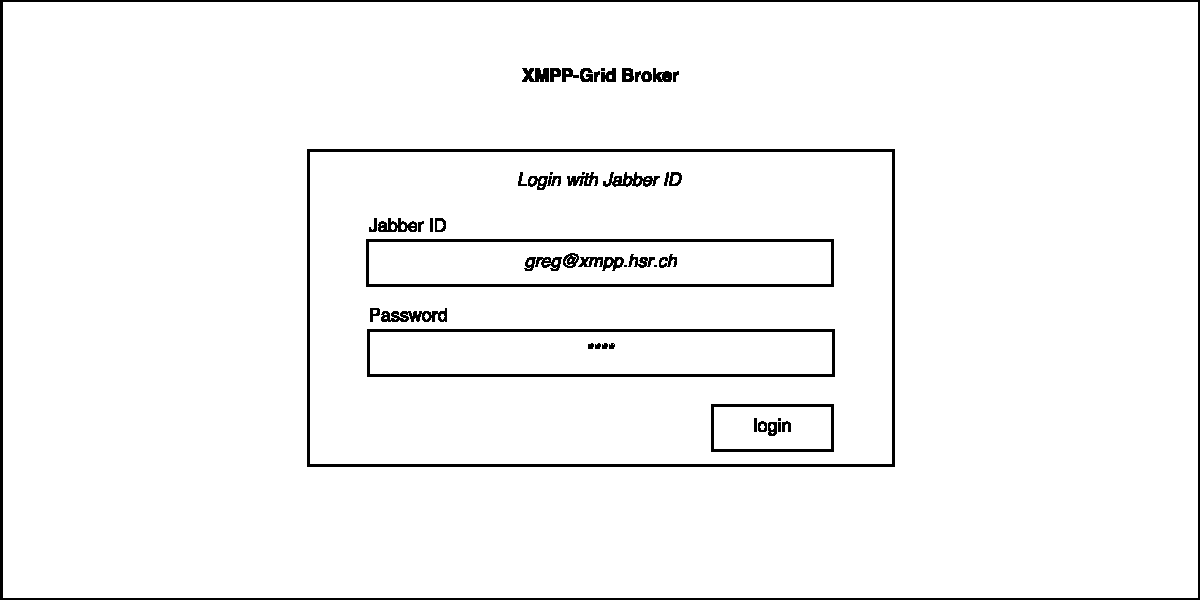
\includegraphics[width=1\linewidth]{resources/wireframe_1}
    \caption{Login-Screen Wireframe}
\end{figure}

\begin{figure}[h]
    \centering
    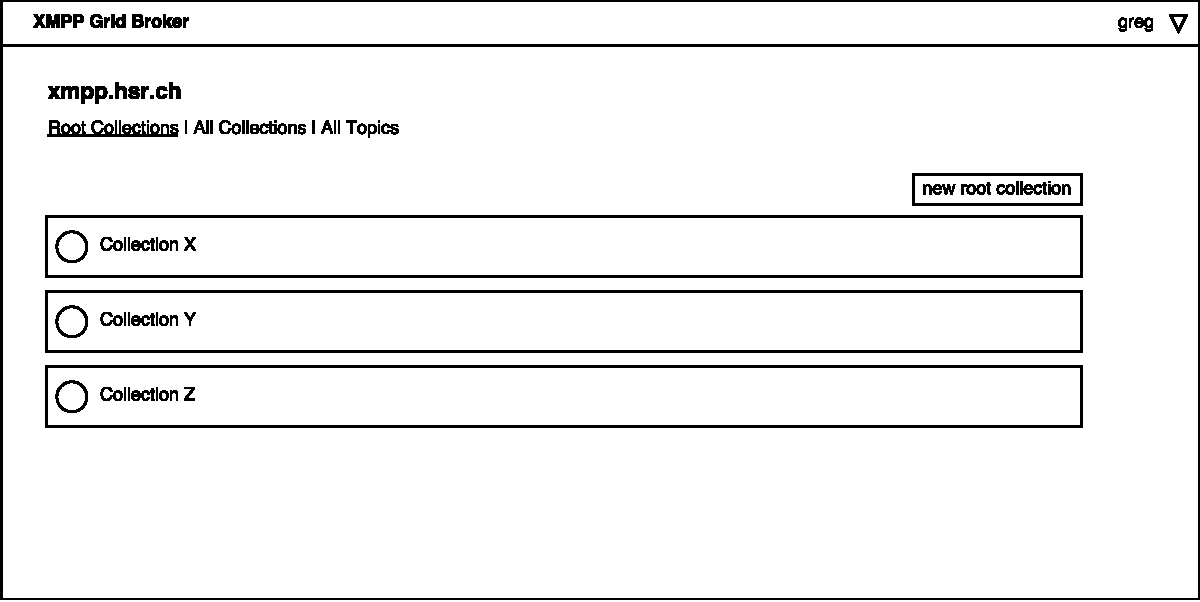
\includegraphics[width=1\linewidth]{resources/wireframe_2}
    \caption{Controller Overview Wireframe}
\end{figure}

\begin{figure}[h]
    \centering
    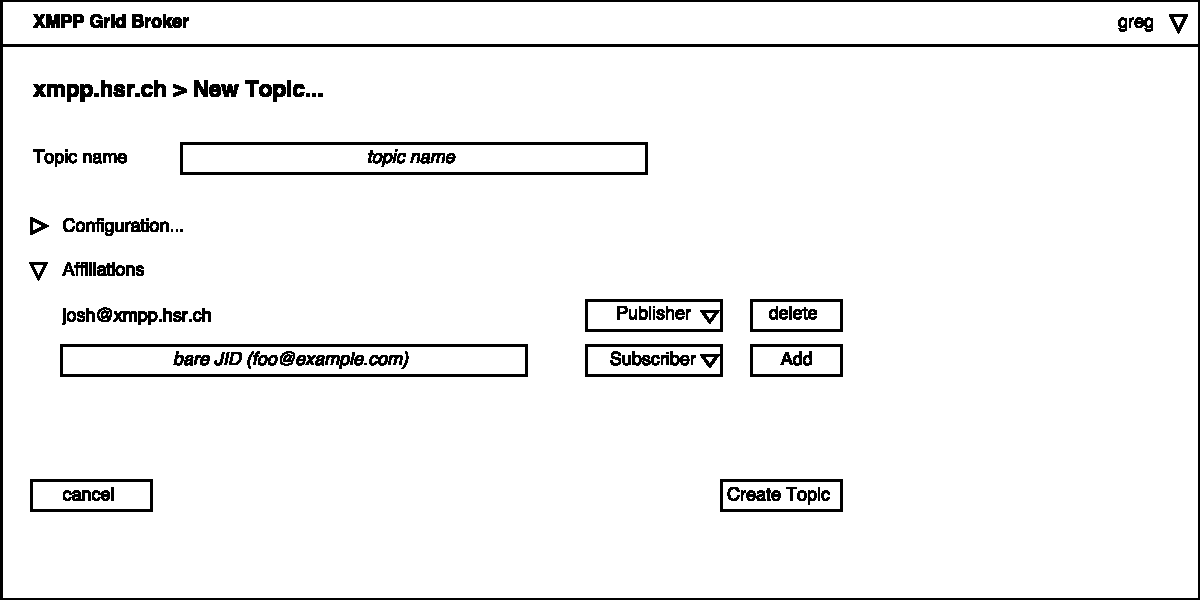
\includegraphics[width=1\linewidth]{resources/wireframe_3}
    \caption{All Collections Wireframe}
\end{figure}

\begin{figure}[h]
    \centering
    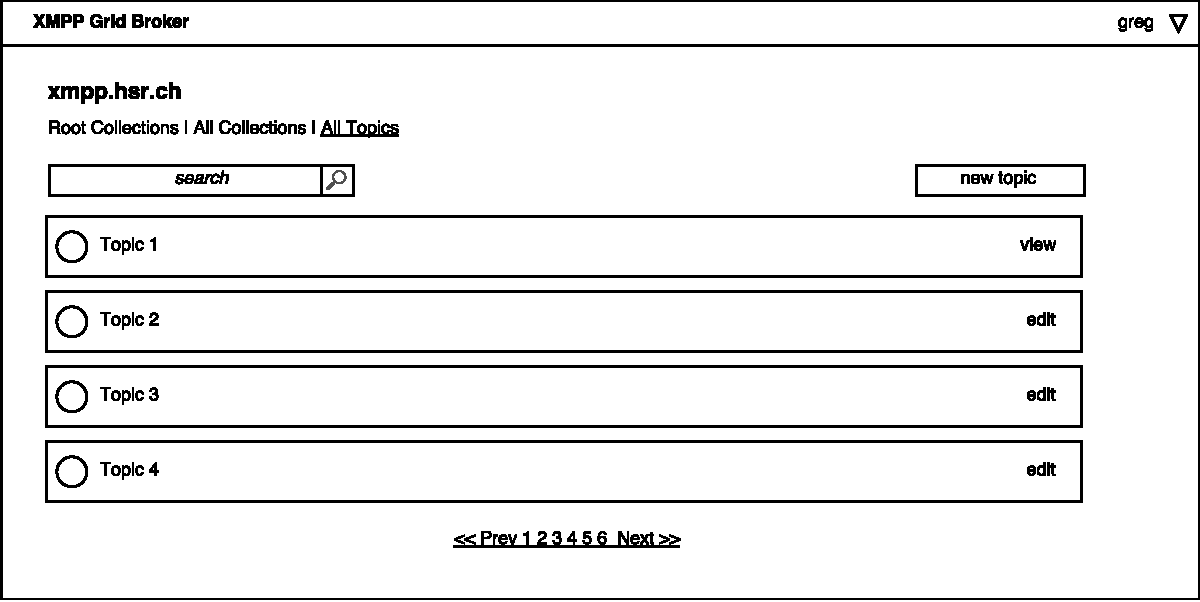
\includegraphics[width=1\linewidth]{resources/wireframe_4}
    \caption{All Topics Wireframe}
\end{figure}

\begin{figure}[h]
    \centering
    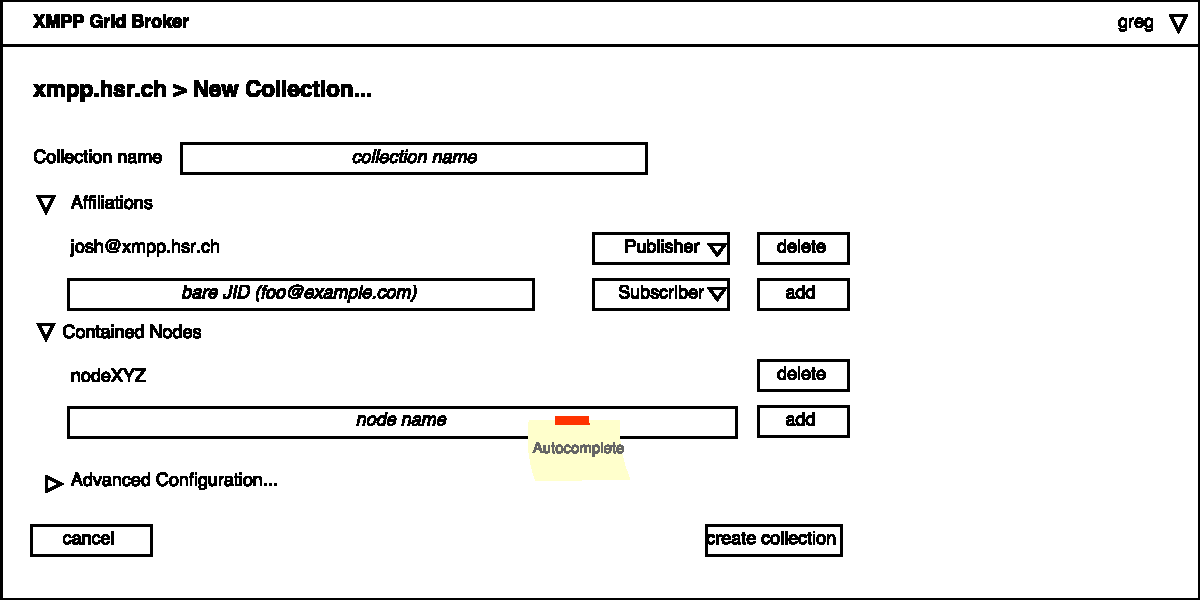
\includegraphics[width=1\linewidth]{resources/wireframe_5}
    \caption{New Collection Wireframe}
\end{figure}

\begin{figure}[h]
    \centering
    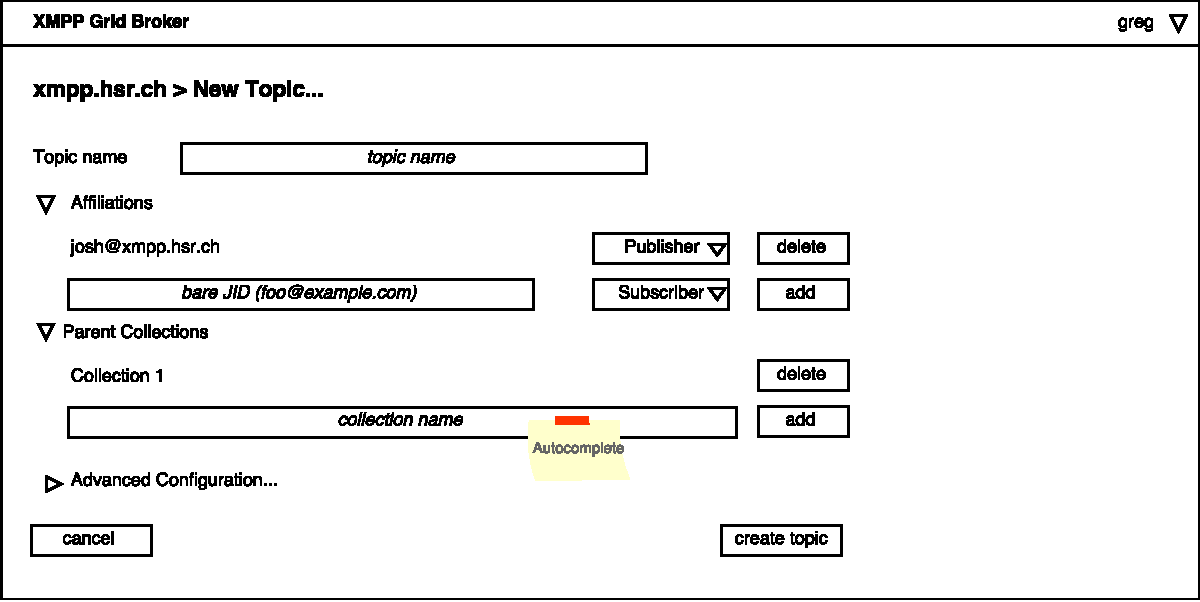
\includegraphics[width=1\linewidth]{resources/wireframe_6}
    \caption{New Topic Wireframe}
\end{figure}

\begin{figure}[h]
    \centering
    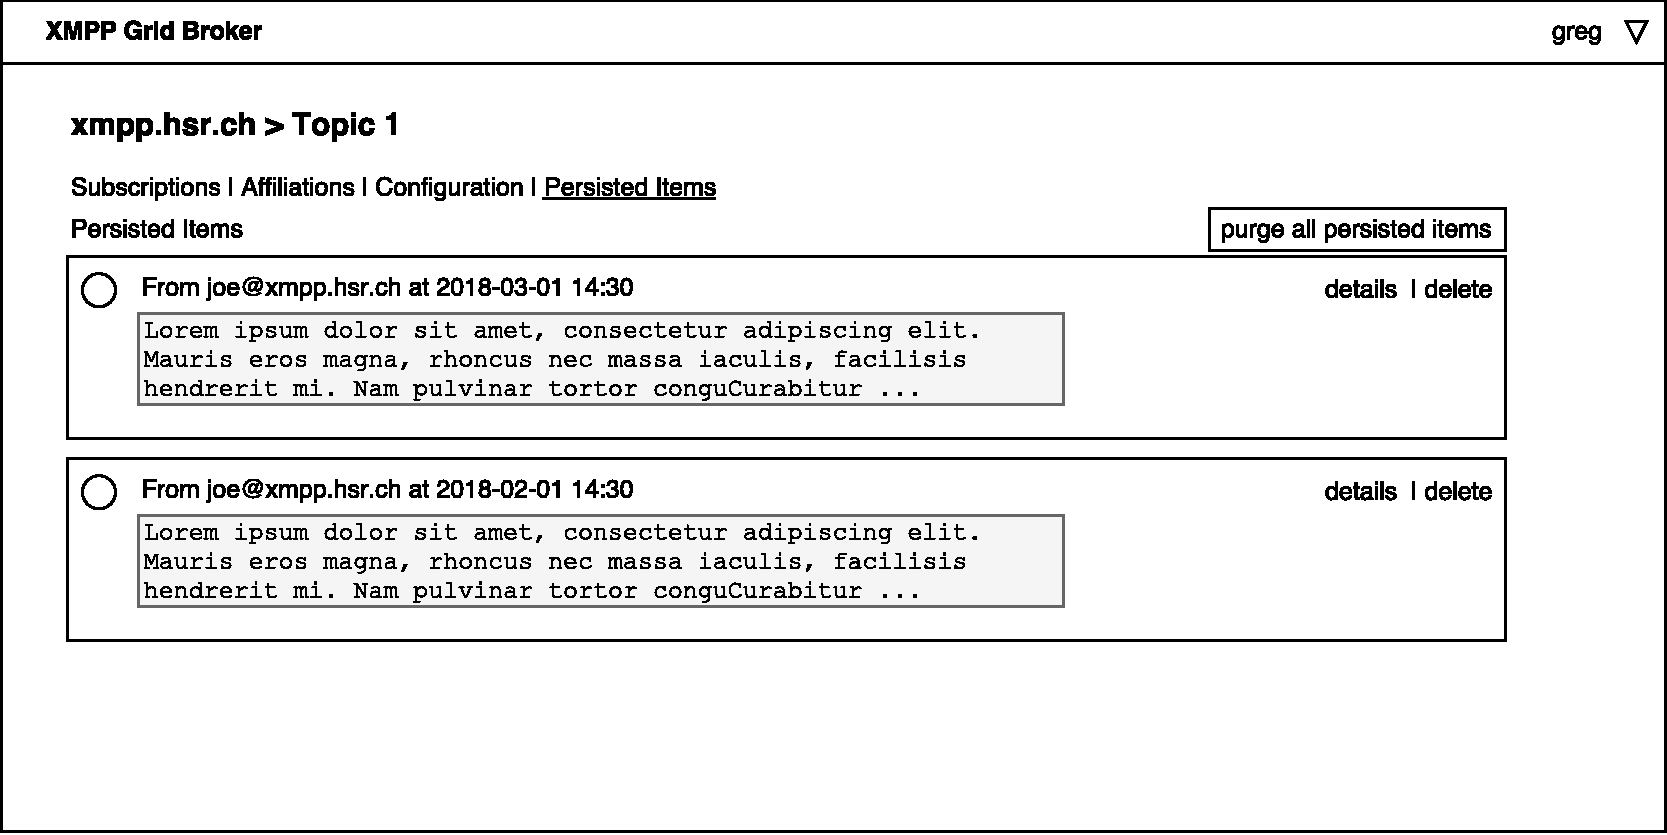
\includegraphics[width=1\linewidth]{resources/wireframe_7}
    \caption{Collection Overview Wireframe}
\end{figure}

\begin{figure}[h]
    \centering
    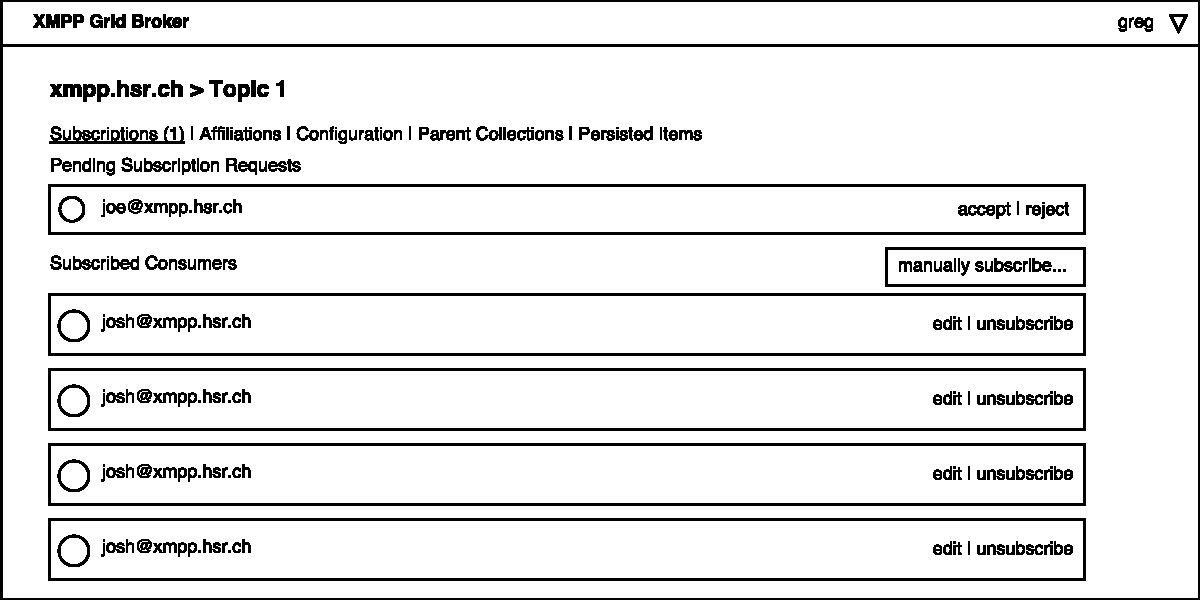
\includegraphics[width=1\linewidth]{resources/wireframe_8}
    \caption{Topic Overview Wireframe}
\end{figure}

\begin{figure}[h]
    \centering
    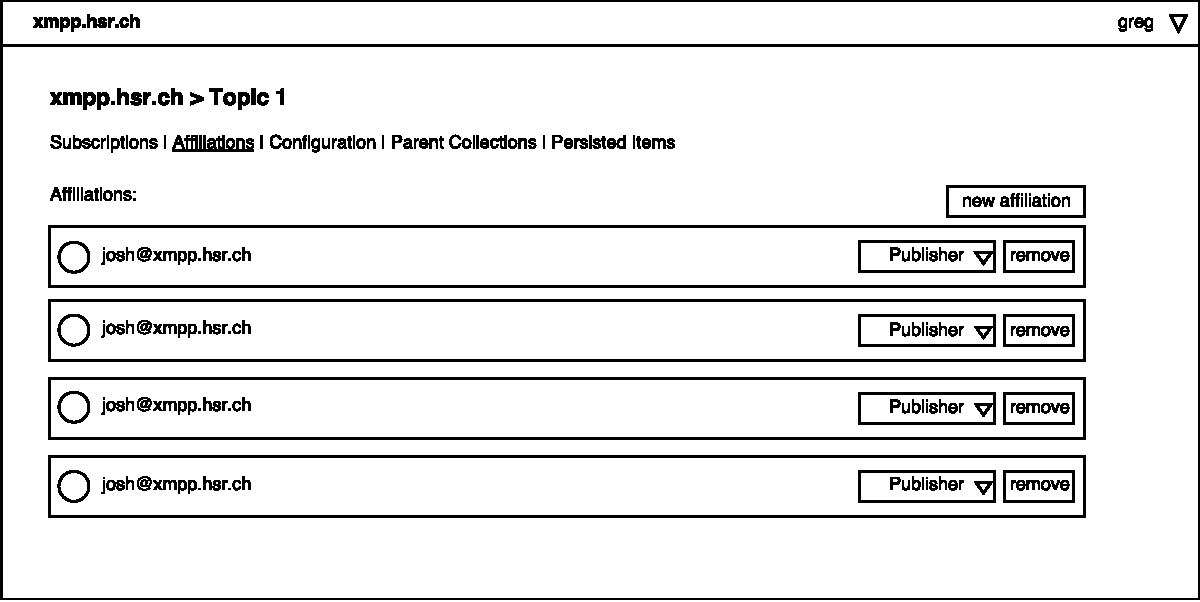
\includegraphics[width=1\linewidth]{resources/wireframe_9}
    \caption{Topic/Collection Affiliations Wireframe}
\end{figure}

\begin{figure}[h]
    \centering
    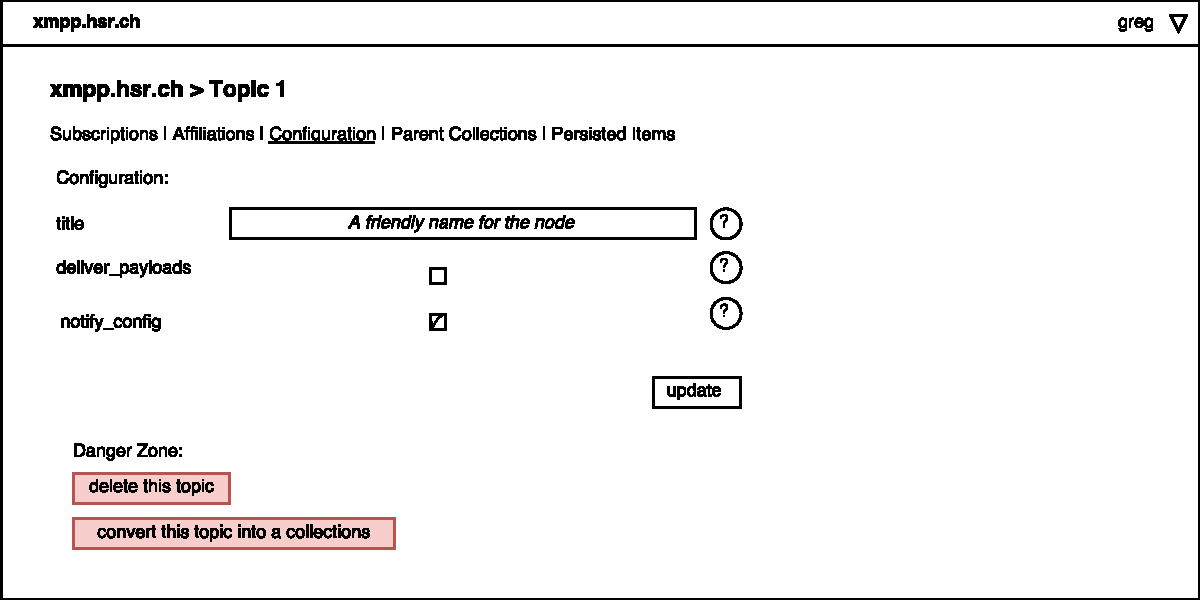
\includegraphics[width=1\linewidth]{resources/wireframe_10}
    \caption{Topic/Collection Configuration Wireframe}
\end{figure}

\begin{figure}[h]
    \centering
    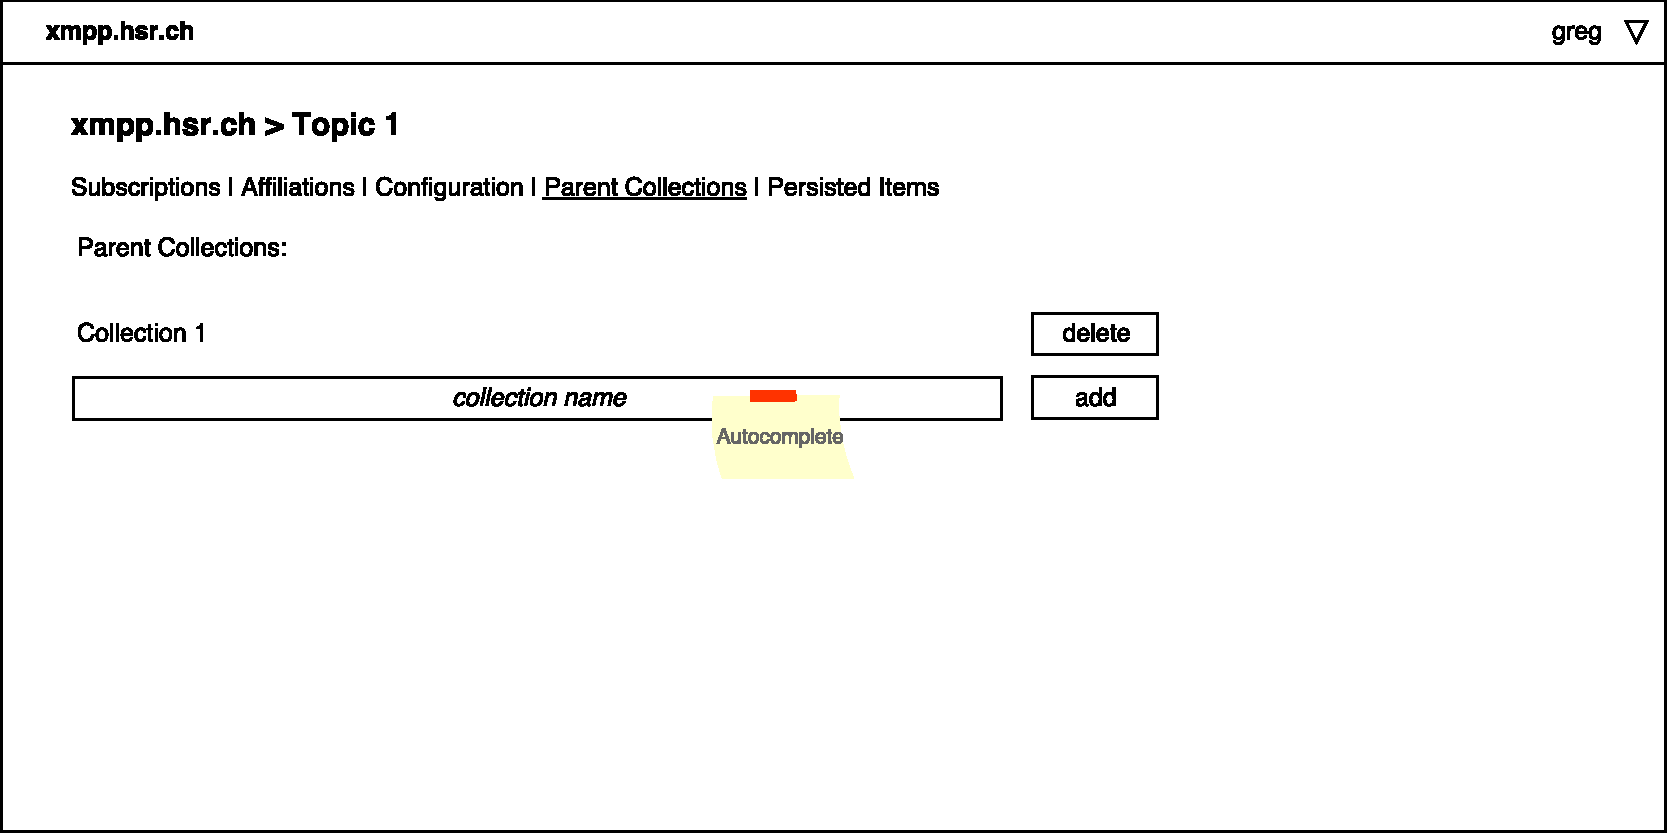
\includegraphics[width=1\linewidth]{resources/wireframe_11}
    \caption{Topic Parent Collections Items Wireframe}
\end{figure}

\begin{figure}[h]
    \centering
    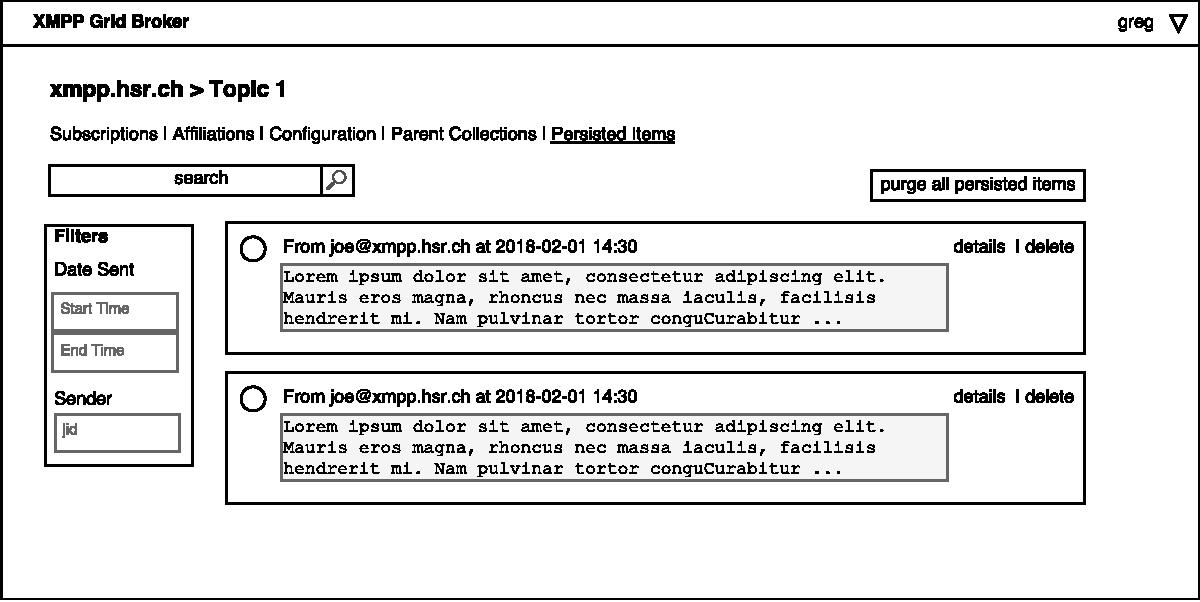
\includegraphics[width=1\linewidth]{resources/wireframe_12}
    \caption{Persisted Items Wireframe}
\end{figure}
% !TeX spellcheck = en_GB
\section{Comparison of XMPP Server and Libraries}\label{sec:comparison-of-xmpp-server-and-libraries}


\subsection{Server}

To find a suited server to develop, test and document our application with, we considered the three major open source \gls{xmpp} servers, which are still under active maintenance and provide extensive documentation on their XEP-implementations.

For our implementation, we might require the following XEPs respectively RFCs. Any deviations are noted under ``XEP/RFC Support''.

\begin{description}
    \item[XEP-0004] Data Forms
    \item[XEP-0030] Service Discovery
    \item[XEP-0059] Result Set Management
    \item[XEP-0060] Publish-Subscribe
    \item[XEP-0114] Jabber Component Protocol
    \item[XEP-0133] Service Administration
    \item[XEP-0178] Best Practices for Use of \gls{sasl-external} with Certificates
    \item[XEP-0206] \gls{xmpp} Over BOSH
    \item[XEP-0248] PubSub Collection Nodes
    \item[RFC-7395] An \gls{xmpp} Subprotocol for WebSocket
\end{description}

\subsubsection{Openfire}
\begin{tabu}{l X}
    Programming Language
    & Java \\

    Plugin Architecture
    & Java JAR\footnote{\url{http://download.igniterealtime.org/openfire/docs/latest/documentation/plugin-dev-guide.html}} \\

    XEP/RFC Support
    & \begin{tabu}{@{}l X}
    XEP-0133 & Partial, also not explicitly supported\footnote{\url{https://issues.igniterealtime.org/browse/OF-284}}\\
    XEP-0178 & Partial, also not explicitly supported\footnote{\url{https://github.com/Connectify/Openfire/blob/master/src/java/org/jivesoftware/openfire/net/SASLAuthentication.java} and \hfill\\ \url{https://issues.igniterealtime.org/browse/OF-1191}}\\
    XEP-0248 & Partial, as part of outdated XEP-0060\footnote{\url{https://igniterealtime.jiveon.com/thread/38929}} \\
    \end{tabu}
    All other required XEPs are supported\footnote{\url{http://download.igniterealtime.org/openfire/docs/latest/documentation/protocol-support.html}}\\

\end{tabu}

\subsubsection{Prosody}
\begin{tabu}{l X}
    Programming Language
    & Lua \\

    Plugin Architecture
    & Luascript\footnote{\url{https://prosody.im/doc/developers/modules}} \\

    XEP/RFC Support
    & \begin{tabu}{@{}l X}
    XEP-0059 & Not supported\\
    XEP-0178 & Not supported\\
    XEP-0248 & Not supported\\
    \end{tabu}
    All other required XEPs are supported\footnote{\url{https://prosody.im/doc/modules} and  \url{https://prosody.im/doc/xeplist}}\\
\end{tabu}

\subsubsection{Ejabberd}
\begin{tabu}{l X}
    Programming Language
    & Erlang \\

    Plugin Architecture
    & Erlang/Elixir\footnote{\url{https://docs.ejabberd.im/developer/extending-ejabberd/modules/}} \\

    XEP/RFC Support
    & \begin{tabu}{@{}l X}
    XEP-0178 & Partial, commercially only\footnote{Server to server only in community edition}\\
    RFC-7395 & Partial, not explicitly supported\footnote{\url{https://docs.ejabberd.im/xmpp}}\\
    \end{tabu}
    All other required XEPs are supported\footnote{\url{http://www.ejabberd.im/protocols}} \\
\end{tabu}

\subsection{Libraries}

To find a suited library to implement our application with, we considered various open source \gls{xmpp} libraries, which are still under active maintenance and provide extensive documentation on their XEP-implementations. We also limited the programming languages to Python, Java and JavaScript as discussed in the project meeting of 2018-03-05 (see~\fullref{sec:meeting-minutes}).

For our implementation, we might require the following XEPs. Any deviations are noted under ``Limitations''.

\begin{description}
    \item[XEP-0004] Data Forms
    \item[XEP-0030] Service Discovery
    \item[XEP-0059] Result Set Management
    \item[XEP-0060] Publish-Subscribe
    \item[XEP-0114] Jabber Component Protocol
    \item[XEP-0133] Service Administration
    \item[XEP-0178] Best Practices for Use of \gls{sasl-external} with Certificates
    \item[XEP-0206] \gls{xmpp} Over BOSH
    \item[XEP-0248] PubSub Collection Nodes
    \item[RFC-7395] An \gls{xmpp} Subprotocol for WebSocket (mentioned only if differs from XEP-0206 implementation status)
\end{description}

\begin{tabu}{l|l l X}
    \hline
    Name
    & Language
    & Plugins
    & Limitations
    \\ \hline

    SleekXMPP\footnote{\url{http://sleekxmpp.com/xeps.html}}
    & Python 2
    & Yes\footnote{\url{http://sleekxmpp.com/create_plugin.html}}
    & \textbf{Not Supported:} XEP-114, XEP-133, XEP-248, XEP-0206\newline
    \textbf{Partial:} XEP-0060\footnote{Client-side only}
    \\

    SliXMPP\footnote{\url{https://github.com/poezio/slixmpp/blob/master/docs/xeps.rst}}
    & Python 3
    & Yes\footnote{\url{https://github.com/poezio/slixmpp/blob/master/docs/create_plugin.rst}}
    & \textbf{Not Supported:} XEP-114, XEP-133, XEP-248, XEP-0206\newline
    \textbf{Partial:} XEP-0060\footnote{Client-side only}
    \\

    aioxmpp\footnote{\url{https://docs.zombofant.net/aioxmpp/devel/\#from-xmpp-extension-proposals-xeps}}
    & Python 3.4
    & Yes\footnote{\url{https://docs.zombofant.net/aioxmpp/devel/api/public/index.html\#apis-mainly-relevant-for-extension-developers}}
    & \textbf{Not Supported:} XEP-0114, XEP-0133, XEP-0178, XEP-248, XEP-0206
    \\

    Smack\footnote{\url{https://download.igniterealtime.org/smack/docs/latest/documentation/extensions/index.html}}
    & Java
    & Yes\footnote{\url{https://github.com/igniterealtime/Smack/tree/master/documentation}}
    & \textbf{Not Supported:} XEP-0114, XEP-0206
    \\

    Babbler\footnote{\url{https://sco0ter.bitbucket.io/babbler/xeps.html}}
    & Java
    & Yes\footnote{\url{https://sco0ter.bitbucket.io/babbler/customextensions.html}}
    & \textbf{Not Supported:} XEP-0133, XEP-0248
    \\

    XMPP-FTW\footnote{\url{http://docs.xmpp-ftw.org/manual/}}
    & JS(Browser)
    & Yes\footnote{\url{http://docs.xmpp-ftw.org/}}
    & \textbf{Not Supported:}\newline XEP-0114, XEP-0133, XEP-0248\newline
    \textbf{Unclear:} XEP-0206, XEP-0178\newline
    \textbf{Note:} Requires Server Abstraction
    \\

    Stanza.io\footnote{\url{https://github.com/legastero/stanza.io/blob/master/docs/Supported_XEPs.md}}
    & JS(Browser)
    & Yes\footnote{\url{https://github.com/legastero/stanza.io/blob/master/docs/Create_Plugin.md}}
    & \textbf{Not Supported:}\newline XEP-0114, XEP-0133, XEP-0248\newline
    \textbf{Partial:} XEP-0178\footnote{Not explicitly supported}
    \\

    strophe.js\footnote{\url{https://github.com/strophe/strophejs-plugins}}
    & JS(Browser)
    & Yes\footnote{\url{https://github.com/strophe/strophejs-plugins}}
    & \textbf{Not Supported:}\newline XEP-0114, XEP-0133, XEP-0248\newline
    \textbf{Partial:} XEP-0178\footnote{Not explicitly supported}
\end{tabu}


%----------------------------------------------------------------------------------------
%	DECLARATION PAGE
%----------------------------------------------------------------------------------------

\begin{declaration}
\addchaptertocentry{\authorshipname} % Add the declaration to the table of contents
\noindent We, \authorname, declare that this thesis and the work presented in it are our own, original work.  All the sources we consulted and cited are clearly attributed. We have acknowledged all main sources of help. \\

\noindent Fabian Hauser\\[2em]
\rule[0.5em]{25em}{0.5pt}\\ % This prints a line for the signature
\noindent Raphael Zimmermann\\[2em]
\rule[0.5em]{25em}{0.5pt}\\ % This prints a line for the signature 
\noindent Rapperswil, \today
\end{declaration}

\cleardoublepage


%----------------------------------------------------------------------------------------

\end{document}  
